
% ---
% Análise do Modelo
% ---
\chapter{Análise do Modelo}
\label{cap:analise}
% ---
    \section{Análise do modelo} 
    \label{sec:model_analysis}
	    A seguir, focamos em uma topologia totalmente conectada. Neste caso, por simetria temos que
        \begin{align}
            \tilde{\pi}(i) &= \binom{N}{i}  \left( \frac{\lambda(N)}{\mu} \right)^{i} \gamma^{i(i-1)/2}, \quad i=0, \ldots, N
        \end{align}
    	A probabilidade de infecção de um nó aleatório escolhido de uma distribuição uniforme dos nós:
    	\begin{equation}
    		{\rho}(N) = \frac{1}{N}    \sum\limits_{i=0}^{N} i \frac{\tilde{\pi}(i)}{{Z}}  
    		\label{eq:rho_N}
    	\end{equation}
	    A análise direta das equações acima é complexa, por envolver um termo quadrático no expoente de $\gamma$.  Para simplificar a análise,  consideramos  uma solução aproximada para o modelo acima. Para tal, definimos $\hat\rho(N) \approx \rho(N)$ e $\hat\pi(i) \approx \tilde\pi(i)$, 
	    \begin{align}
            \hat{\rho}(N) &= \frac{1}{N} \sum\limits_{i=0}^{N} i \frac{\hat{\pi}(i)}{{\hat Z}}\label{eq:rho_Nhat2} \\
            \hat{\pi}(i)  &= \binom{N}{i} \left(\frac{\lambda(N)}{\mu}\gamma^{N^{\star}/2}\right)^{i} \label{eq:tilde_pi_i} \\
            \hat{Z} &= \sum\limits_{i=0}^{N} \hat{\pi}(i) \label{eq:tilde_hat_z}
        \end{align}
		onde $N^{\star}(N)$ é uma função crescente de $N$, que denotamos simplesmente por $N^{\star}$ para simplificar a notação.  Nos referimos a o modelo proposto para aproximar a solução do modelo original como \textit{aproximação binomial}, por fazermos uso do binômio de Newton na demonstração do resultado a seguir: 

        \begin{lemma}
        No modelo binomial,  temos que 
        	\begin{equation}
				\hat{\rho}(N) =   \frac{1}  {1+ \mu/(\lambda(N) \gamma^{N^{\star}/2} )  } \\
        	\end{equation}
        \end{lemma}	
        \begin{proof}	
            O resultado é fruto de manipulações algébricas,
            \begin{align}
            \hat{Z} \hat{\rho}(N) &= \frac{1}{N} \sum_{i=0}^N i \binom{N}{i} \left( \frac{\lambda(N)}{\mu}\gamma^{N^{\star}/2} \right)^i = \sum_{i=1}^N\binom{N-1}{i-1}\left(\frac{\lambda(N)}{\mu}\gamma^{N^{\star}/2}\right)^i \label{eq:binom_mirror} \\
            &= \color{black}{\left(\frac{\lambda(N)}{\mu}\gamma^{N^{\star}/2}\right)\left(1+\frac{\lambda(N)}{\mu}\gamma^{N^{\star}/2}\right)^{N-1}} \label{eq:thm_binom} %\tag{3}
            \end{align}
            O resultado segue a partir da obtenção, de forma similar, da  expressão de $\hat{Z}$. 
        \end{proof}
        O resultado acima pode ser usado, por exemplo, para caracterizarmos os pontos de equilíbrio do sistema.

        \begin{thm}
            O modelo binomial admite no máximo dois equilíbrios interiores ao considerarmos um custo de vacinação constante, desde que $\gamma>1$, $\partial N^{\star}/\partial N$ seja positivo e não decrescente e $\lambda(N)$ decrescente.     \label{thm:main}
        \end{thm}
        \begin{proof}
            Seja $\tau(N)= (\lambda(N)/\mu)\gamma^{N^{\star}/2}$. Então, pelo lema acima, temos que $\partial \hat \rho(N)/\partial N =  (\partial \tau/\partial N)/(\tau^2 (1+1/\tau)^2)$. Claramente, todos os termos de $\partial \hat \rho(N)/\partial N$ são positivos, com exceção de $\partial \tau/\partial N$.  Temos que
            \begin{equation}
            \frac{\partial \tau}{\partial N} = \lambda(N) \gamma^{N^{\star}/2} \left(\frac{1}{2} \log \gamma  \frac{\partial N^{\star}}{\partial N} + \frac{\lambda'(N)}{\lambda(N)}   \right)
            \end{equation}
            Se $ \frac{\partial N^{\star}}{\partial N} $ for positivo e não decrescente, e $\lambda(N)$  for decrescente, a expressão acima admite um único zero.  Assim, a função $\hat \rho(N)$ possui no máximo um ponto de mínimo interno, e por isso cruza qualquer linha horizontal em no máximo dois pontos.   
        \end{proof}
        O resultado acima está de acordo com a ilustração apresentada nas Figuras~\ref{fig:result_01b}~e~\ref{fig:equilibrim_cost}. Segundo a Figura~\ref{fig:result_01b}, em todos os casos em que $\gamma > 1$, a probabilidade de um nó estar infectado primeiro diminui e depois aumenta, ou simplesmente sempre aumenta.  Conforme discutido na Figura~\ref{fig:equilibrim_cost}, a um ponto de mínimo correspondem dois equilíbrios, um estável e um instável. 

        \paragraph*{Caso especial: $\lambda(N)=\Lambda/N$}
        O modelo proposto é factível de análise em fórmula fechada para vários casos especiais da função $\lambda(N)$. Para fins de ilustração, consideramos o caso especial em que $\lambda(N)=\Lambda/N$.  Este caso corresponde a um atacante que tem poder de ataque (\emph{budget}) constante igual a $\Lambda$ infecções por segundo, e divide esse poder entre os $N$ nós da rede. Nesse caso, $\lambda' (N) = -\Lambda/N^2$. Assumindo para fins de simplificação que  $N^{\star}=N$, temos
		\begin{equation}
			\frac{\partial}{\partial N}\hat{\rho}(N)  = \kappa \left( \frac{1}{2} \log \gamma - \frac{1}{N} \right)
		\end{equation}
		onde $\kappa$ é uma constante positiva. 
		Podemos verificar que $\frac{\partial}{\partial N}\hat{\rho}(N)=0$ quando $N = (2 / \log \gamma)$. % para valores $N < (2 / \log \gamma)$ a derivada é negativa, e valores $N > (2 / \log \gamma)$ a derivada é positiva. 
		No caso de $\gamma = 1.09$ encontramos o valor crítico quando $N \approx 23$, que está de acordo com aquele apresentado na Figura~\ref{fig:result_01b}. 

        Note também que podemos obter fórmulas fechadas para os pontos de equilíbrio.
        Para tal, seja $C$ o custo de aplicação da contramedida.  Então, os pontos de equilíbrio interno são pontos tais que $\hat{\rho} (N) - C = 0$. 
		Assumindo para fins de simplificação que  $N^{\star}=N$, temos que 
		os valores de $N$ que satisfazem a equação de equilíbrio são  
		$N = \frac{-2}{\log \gamma}    W \left(\frac{\Lambda (C-1) \log\gamma}{2C \gamma^{1/2} }  \right)$ 
		onde $W(x)$ é a função de Lambert, que admite dois valores reais, correspondentes aos ramos -1 e 0.  
		No caso de $\Lambda = 10$, $\gamma = 1,09$ e $C = 0.6$, por exemplo, temos os valores de $N$ correspondentes aos ramos $-1$ e $0$  dados por 45,6 e  9,7.  O segundo equilíbrio condiz com o  resultado da   Figura~\ref{fig:equilibrim_cost}, enquanto que o primeiro foi superestimado. Tal fato deve-se à simplificação de que $N^{\star}=N$, conforme ilustrado na Figura~\ref{fig:result_01b}, podendo o resultado ser melhor aproximado em refinamentos sucessivos do modelo. 
		A Figura~\ref{fig:result_01b}(a) mostra a probabilidade de um nó estar infectado, em função do número de nós na rede.  A aproximação $N^{\star}=N$ captura bem o comportamento do sistema antes de $\rho(N)$ atingir o seu ponto de mínimo. Depois deste ponto, é necessário ajustar $N^{\star}$ para o seu valor ótimo, que é crescente e sempre maior que $N$ como ilustrado na Figura~\ref{fig:result_01b}(b) (satisfazendo os critérios do Teorema ~\ref{thm:main}).  
		De forma mais geral, cabe destacar que o fato de a   função de Lambert possuir dois ramos reais  está de acordo com a constatação de que o sistema admite  no máximo dois equilíbrios internos (vide Teorema~\ref{thm:main}).   

        \begin{figure}[!htb]
    		\centering
    	    \hspace{-0.2in}	
            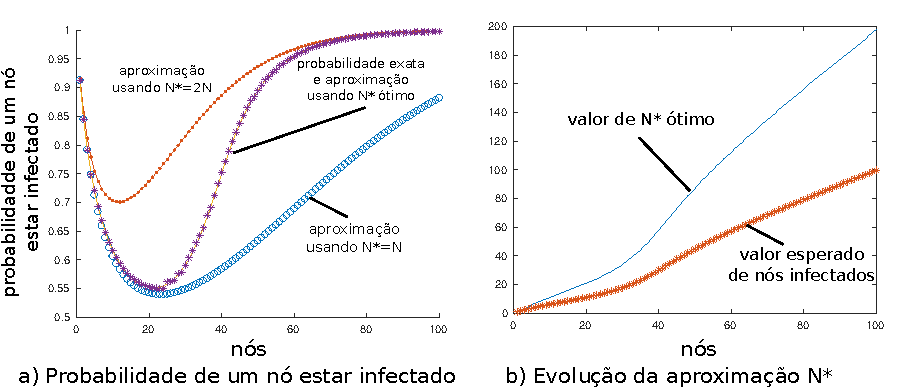
\includegraphics[width=0.99\columnwidth,keepaspectratio=false]{./img/aproximacoes_N_ast.pdf}
    		\caption{Validação da solução aproximada pelo modelo binomial ($\gamma=1,09$).}
    		\label{fig:result_01b}
        \end{figure}
        
        
